% Skala des Zeitschalters (rechter Drehknopf), eigene Zeichnung nach dem Bedienpanel.
% Winkel: off oben (90°), Zeitbetrieb im Uhrzeigersinn 10 ... 60 min,
% Dauerbetrieb (on, unendlich) schon kurz links von off.
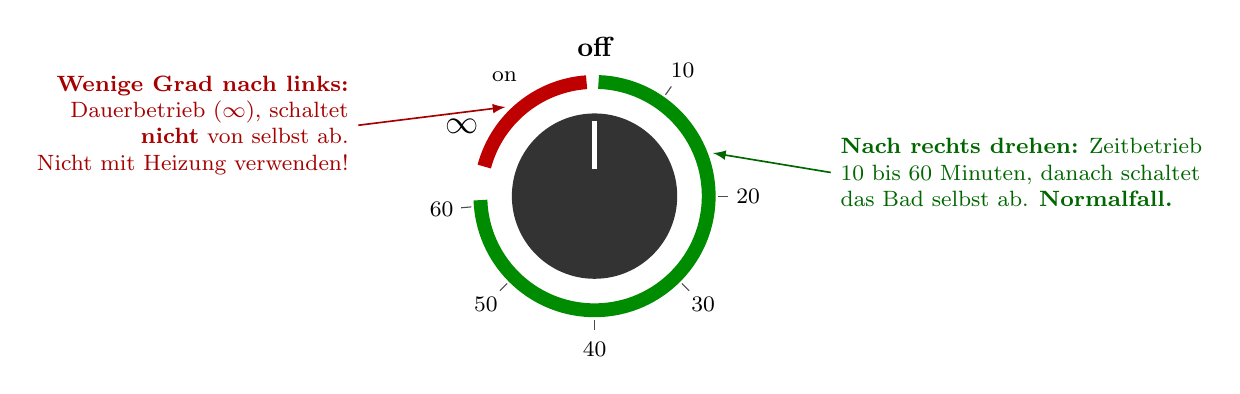
\begin{tikzpicture}[font=\footnotesize]
	\def\R{1.45}
	% Bereiche
	\draw[line width=5pt, green!55!black] (88:\R) arc[start angle=88, end angle=-178, radius=\R];
	\draw[line width=5pt, red!75!black] (94:\R) arc[start angle=94, end angle=165, radius=\R];
	% Drehknopf
	\fill[black!80] (0,0) circle (1.05);
	\draw[white, line width=1.5pt] (0,0.35) -- (0,0.95);
	% Skala
	\foreach \w/\t in {55/10, 0/20, -45/30, -90/40, -135/50, 185/60} {
		\draw[black!70] (\w:\R+0.12) -- (\w:\R+0.25);
		\node at (\w:\R+0.5) {\t};
	}
	\node[font=\bfseries] at (90:\R+0.45) {off};
	\node at (127:\R+0.45) {on};
	\node[font=\large] at (152:\R+0.45) {$\infty$};

	% Erklärungen
	\node[align=left, anchor=west, text=green!40!black] (z) at (3.0,0.3)
		{\textbf{Nach rechts drehen:} Zeitbetrieb\\10 bis 60 Minuten, danach schaltet\\das Bad selbst ab. \textbf{Normalfall.}};
	\node[align=right, anchor=east, text=red!65!black] (d) at (-3.0,0.9)
		{\textbf{Wenige Grad nach links:}\\Dauerbetrieb ($\infty$), schaltet\\\textbf{nicht} von selbst ab.\\Nicht mit Heizung verwenden!};
	\draw[-latex, green!40!black, line width=0.6pt] (z.west) -- (20:\R+0.15);
	\draw[-latex, red!65!black, line width=0.6pt] (d.east) -- (135:\R+0.15);
\end{tikzpicture}
